\chapter{Reducing Collection Bloat}

 Relationships in an
entity-relationship model are typically implemented in Java using the
standard library collection classes. While a simple 1:1 relationship can be
implemented with a single map, more complex 1:n, n:1, and m:n are usually 
implemented with collections inside other
collections, sometimes nested three or more levels deep. 
As a result, it is common for a Java application to create hundreds of
thousands, even millions, of collections, where the vast majority have only a
very small number of entries.

Our guess is that the
collection class developers would be surprised by this usage pattern. 
Why would they have bothered implementing expandable
structures and clever hashing algorithms for only a few entries?
This mismatch between collection implementation and usage is 
a leading cause of memory bloat. The basic cost of a collection, even an
empty collection, is remarkably high. Creating millions of small collections
multiplies this basic infrastructure cost, which is all overhead, filling the
heap. This chapter shows
 how to mitigate the many-small-collections problem to reduce memory bloat.
 
 \section{Choosing The Right Collection}

The standard Java collections vary widely in now much memory they use.
Not surprisingly, the more functionality a collection provides, the more
memory it uses. Collections range from a simple, highly efficient
\class{ArrayList} to
\class{ConcurrentHashMap}, which offers sophisticated concurrent access
control, and has extremely large overhead. 
The use of overly general collections, that provide more functionality than
really needed, is a common pattern leading to excessive memory bloat.
Since collection class implementations is hidden, it's
easy to see how this happens.

To illustrate, consider a graph with 100,000 nodes that have four edges each, on
average. An obvious implementation is to use a
\class{HashMap}, where the keys are nodes and the values are \class{HashSets}
of edges. A node is an \class{Integer}, and an edge consists of two
\class{Integers}, a node number and an edge weight.
Figure~\ref{fig:graph-hashset} shows an entity-collection diagram for the graph.
 \begin{figure}
  \centering
 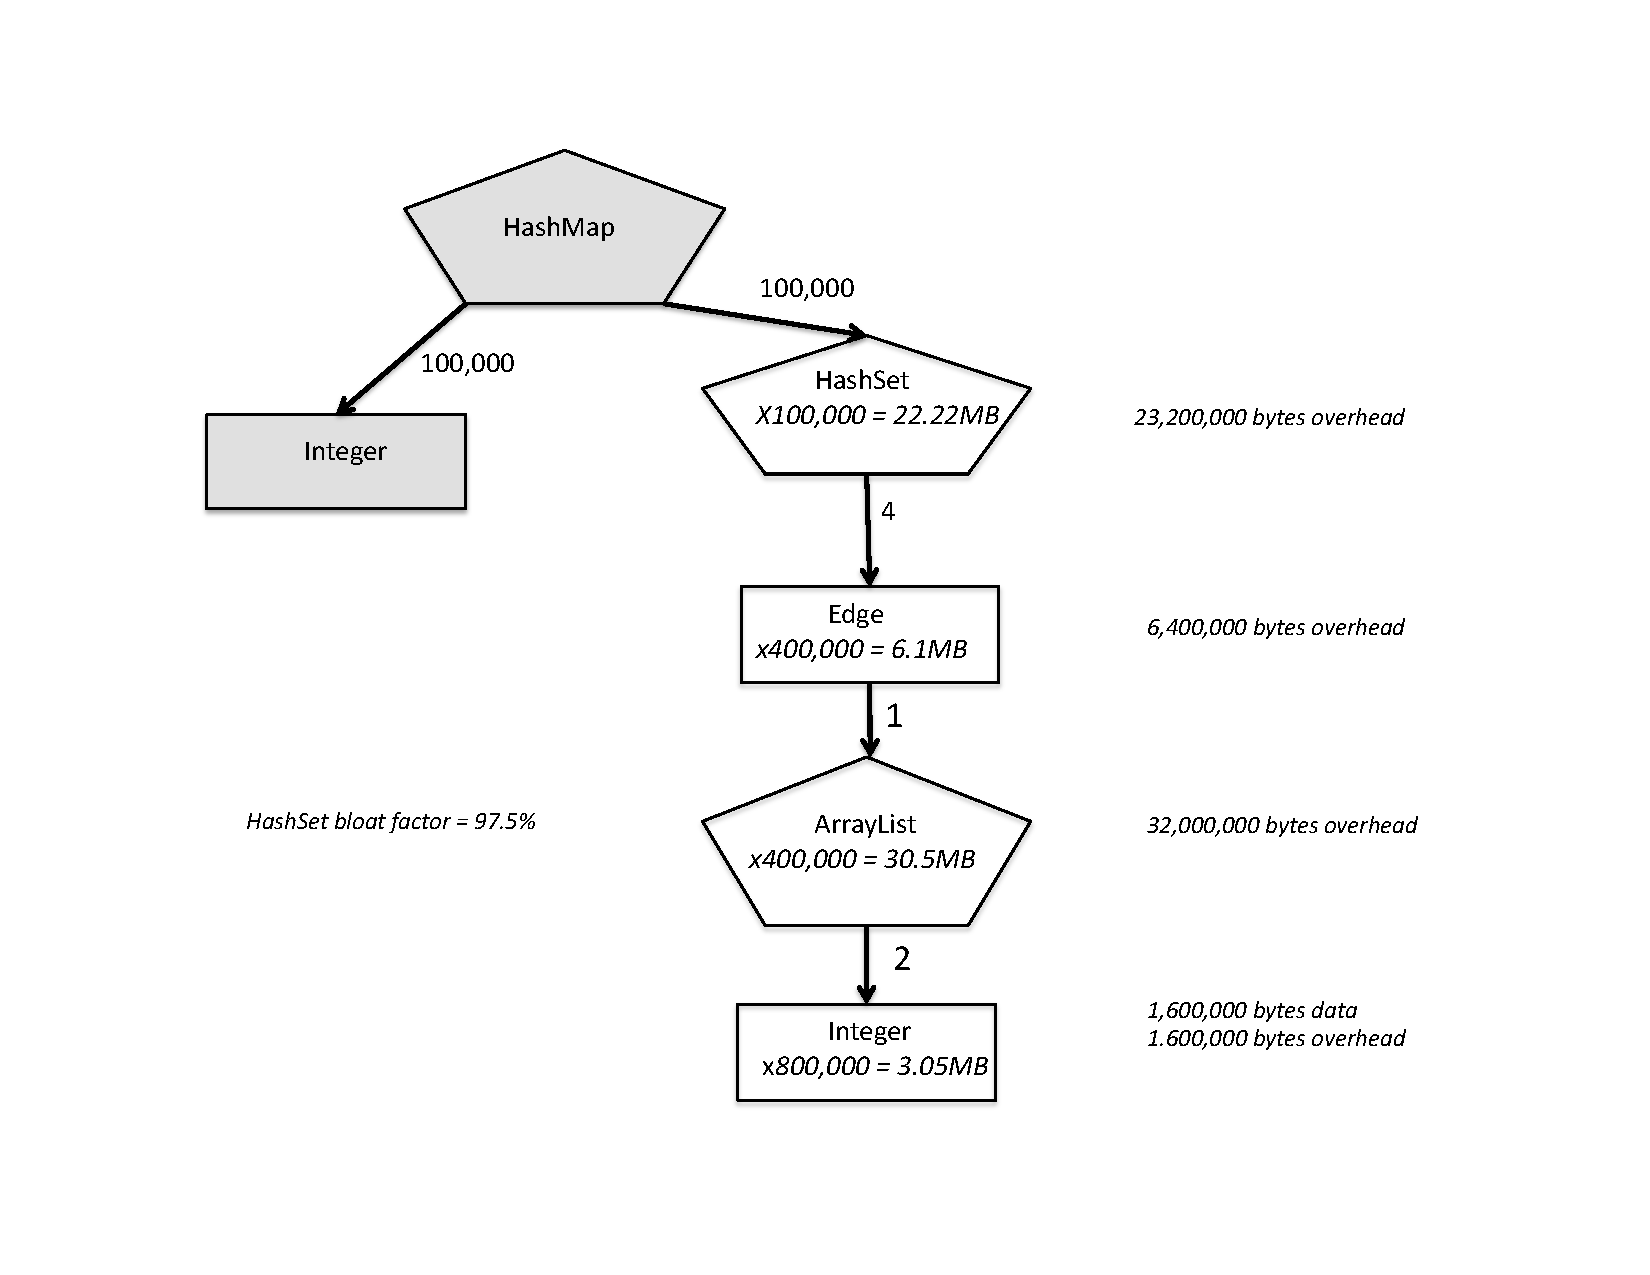
\includegraphics[width=.80\textwidth]{part3/Figures/graph-hashset.pdf}
  \caption{A 100,000-node graph, stored as a
  \class{HashMap} from \class{Nodes} to \class{HashSets} of \class{Edges}.}
  \label{fig:graph-hashset}
\end{figure}
%Sun library --  Empty HashSet -- 136 bytes
% 16 bytes HashSet (header + pointer)
% 40 byptes HashMap Object 
% 80 bytes empty array of entries

%HashMapEntry:  24 bytes:  header + 4 fields (value, key, next, hash)
% 4 entries -- 96 bytes
% total overhead for 4 entry hashset: 232 bytes
% 100,000 hashsets with 4 entries is 22.13MB

% HashMap size: 40 for header + 8 for array header
% 24 bytes per entry + 6 per entry in the array (assume extra for growth space)
% so for 100,000 entries, thats 48 + 3,000,000 bytes = 2.86MB
%
% Edge 16*400,000 = 6.4 million = 6.1MB
%
% ArrayList container is 24 bytes (header, size, modcount, pointer) 
% Default array size os 10 -- 10*4+12 = 52 rounds to 56
% ArrayList is 80 (56+24) for 4 entries.
% 100,000 ArrayLists is: 8,000,000 bytes

There are several bloat problems here. The first problem is that 
 each of the 100,000 very small \class{HashSets} consumes 232 bytes, all
 overhead. It's hard to think of a good reason why such a heavy-weight
 structure should ever be used for storing around four entries, and yet, this is
 a very common pattern. For small sets, \class{ArrayList}
 is almost always a better choice. \class{HashSet} maintains uniqueness
  and provides fast access, but enforcing uniqueness
is not always needed. If uniqueness is
important, it can be easily implemented, 
often without significant performance when lists are small. 
 Figure~\ref{fig:graph-arraylist} shows improved memory usage with
\class{ArrayList}. Each \class{ArrayList} incurs 80 bytes of overhead, almost
a third as much as a \class{HashSet}.

\section{The Cost Of Collections}

Let's look at why a \class{HashSet} is so much bigger than an \class{ArrayList}. 
Some of the \class{HashSet} memory overhead is Java-related and
unavoidable. Other overhead is the result of hard-coded assumptions and design
goals, as shown in~\ref{fig:hashset.pdf}. For example, the
\class{HashSet} implementation assumes \class{HashSets} will be very large, 
and trades memory space in favor of performance. 
Here are the causes of unnecessary \class{HashSet} bloat.
 \begin{figure}
  \centering
 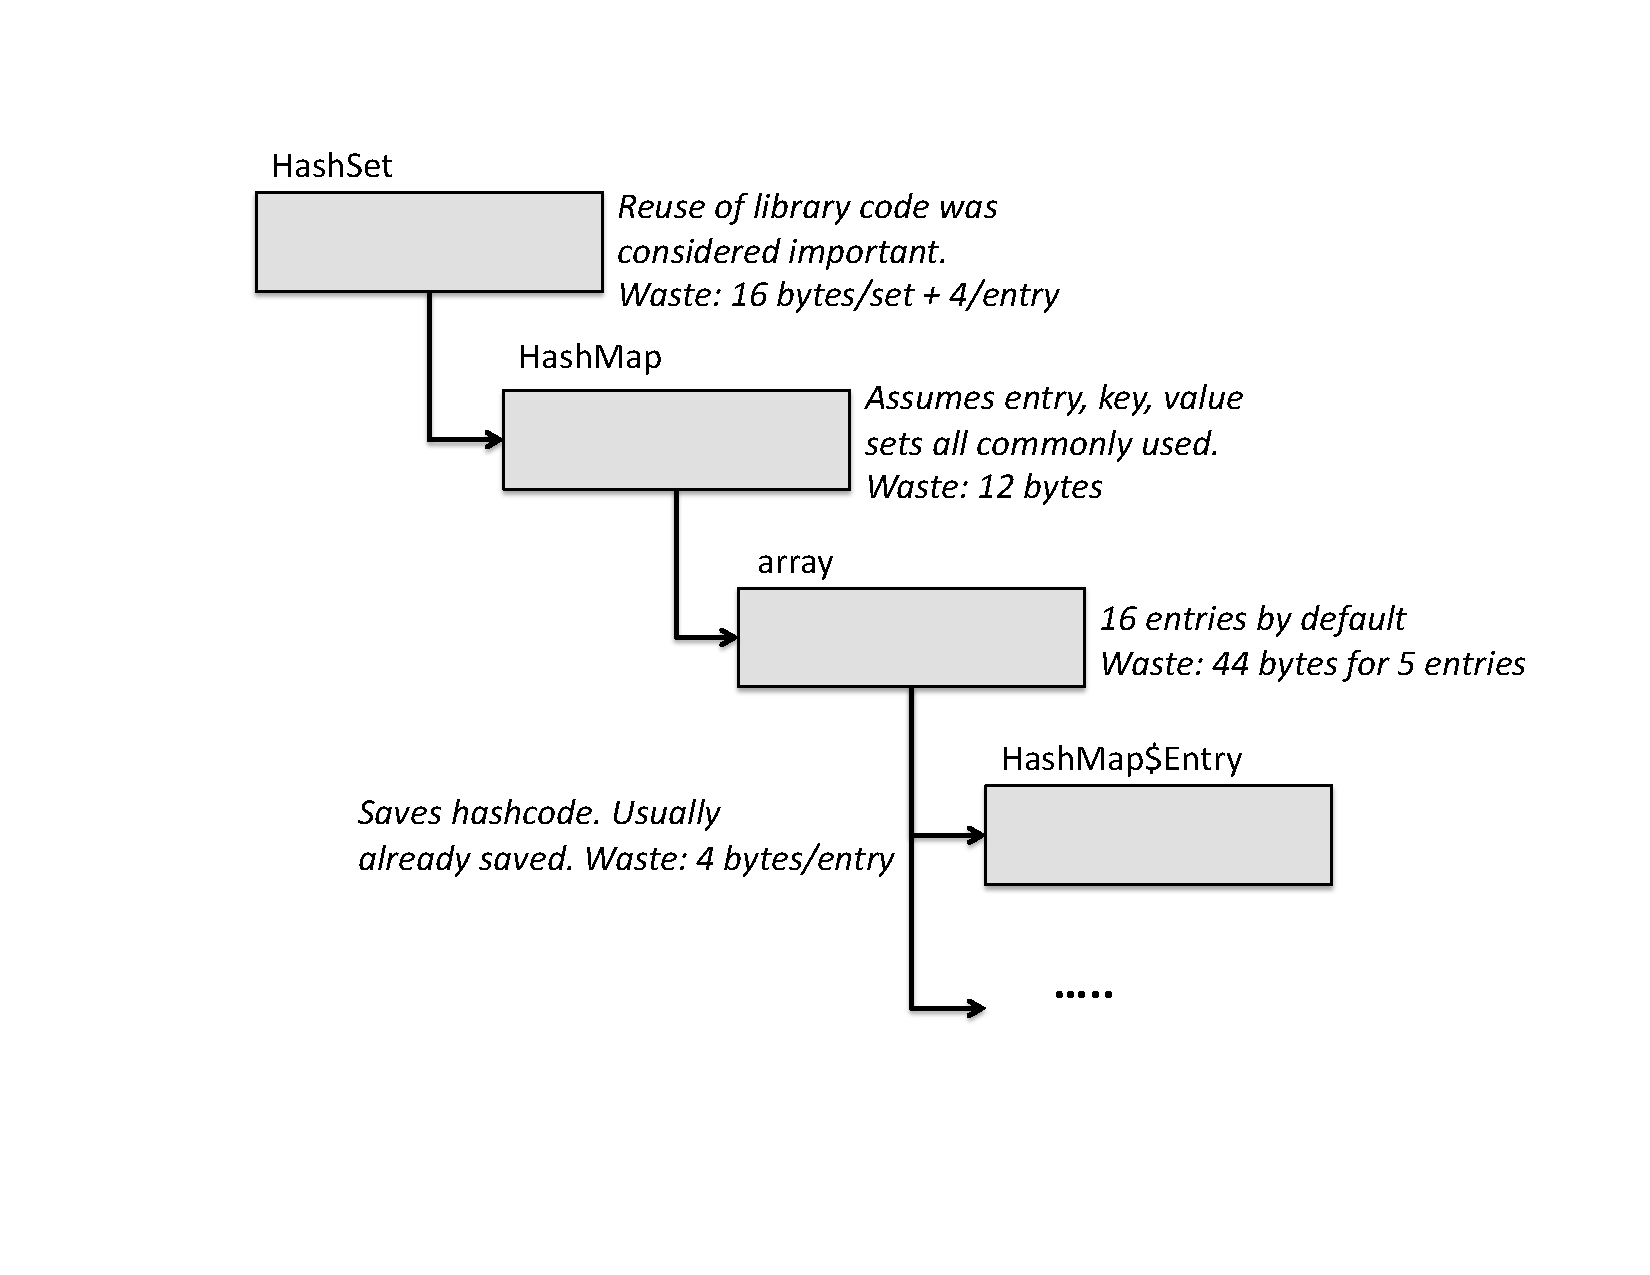
\includegraphics[width=.80\textwidth]{part3/Figures/hashset.pdf}
  \caption{The internal structure of a \class{HashSet} showing how
  implementation assumptions waste memory.}
  \label{fig:hashset}
\end{figure}

\paragraph{Reusing HashMap} Internally, a \class{HashSet} is just a wrapper,
delegating all of its work to a \class{HashMap}.
This decision to reuse the \class{HashMap} code instead of specializing
\class{HashSet} costs an extra 16 bytes, which is reasonable if
\class{HashSets} are big and the fixed overhead costs are amortized away. 
Unfortunately, fixed cost is magnified when there are many
small \class{HashSets}. 
Also, \class{HashMap} is
more general than needed.
Each \class{HashMap\$Entry} stores a key and a
value, and \class{HashSet} only uses the key, so four bytes are wasted per
entry. Sometimes specialization is a better option than reuse, especially for
library classes, where the usage patterns are not known in advance.
  
\paragraph{Open Chaining} \class{HashMap} itself is fairly
 expensive. First, the \class{HashMap} object is just a container pointing
 to the actual array of entries. This delegation is necessary in Java.
 Secondly, \class{HashMap} uses an
 open chaining algorithm, which means that clashing entries are chained in a
 linked list. With open chaining, each entry requires its own
 \class{HashMap\$Entry} object and an extra level of indirection.
 
\paragraph{Default Array Size} 
A \class{HashMap}, which is used to implement a \class{HashSet}, has a default
size of 16 entries, which means that its array of entries has an initial
size of 16. If most \class{HashSets} have only a few entries, this wastes space. 
For example, a \class{HashSet} with five entries wastes 44 bytes.


\paragraph{Bookkeeping Fields} \class{HashMap} allows callers to iterate over its set of keys,
 its set of its
values, and its set of its entries. These sets are cached once they are created.
Every \class{HashMap}, and every \class{HashSet} has three pointers
to store these sets, which is an extra 12 bytes.
However, its not that common to use
any of these sets, and very rare to use more than one set at a time.
 Certainly for \class{HashSet}, 
there is never a need for a set of values.
  
 \paragraph{Extra Per-Entry Costs} Each \class{HashMap\$Entry} stores a
 hashcode, which is an unnecessary redundant field. The most common keys are either
 \class{Strings}, which store their own hashcode, or \class{Integers}, whose
 hashcodes are easy to compute. 

An \class{ArrayList} is much simpler than a
\class{HashSet}. It is really just an expandable array, consisting of a
wrapper object and an array of entries, as shown in Figure~\ref{fig:arraylist}.
 \class{ArrayList} is better than \class{HashSet} in two ways. First, it has a
 lower fixed cost, which means that \class{ArrayLists} with just a few elements
 is smaller than a \class{HashSet} of the same elements. Fixed costs include
 wrapper objects and unitialized array elements. The fact that \class{HashSet}
 delegates to \class{HashMap} dramatically inflates its fixed cost. 
 
 Secondly, \class{ArrayList} has a lower per-entry cost, which means that
 \class{ArrayList} scales much better than \class{HashSet}. The per-entry cost
 of an \class{ArrayList} entry is 4 bytes, the cost of an entry array pointer.
 The per-entry cost of a \class{HashSet} is an array pointer plus a
 \class{HashMap\$Entry}, which is 28 bytes. So \class{ArrayList}  is better
 both for small and large sets.

Table~\ref{tab:collection-costs} shows the empty-collection costs of four basic
collections, \class{ArrayList}, \class{LinkedList}, \class{HashMap}, and \class{HashSet}. These costs have been
calculated based on the the Sun JVM and ?? library, using the techniques
described in Chapter~\ref{}. There various other Java standard library
implementations in circulation have costs
similar to these. You can calculate them by the same methodology as used here.

\begin{table}
  \centering
 %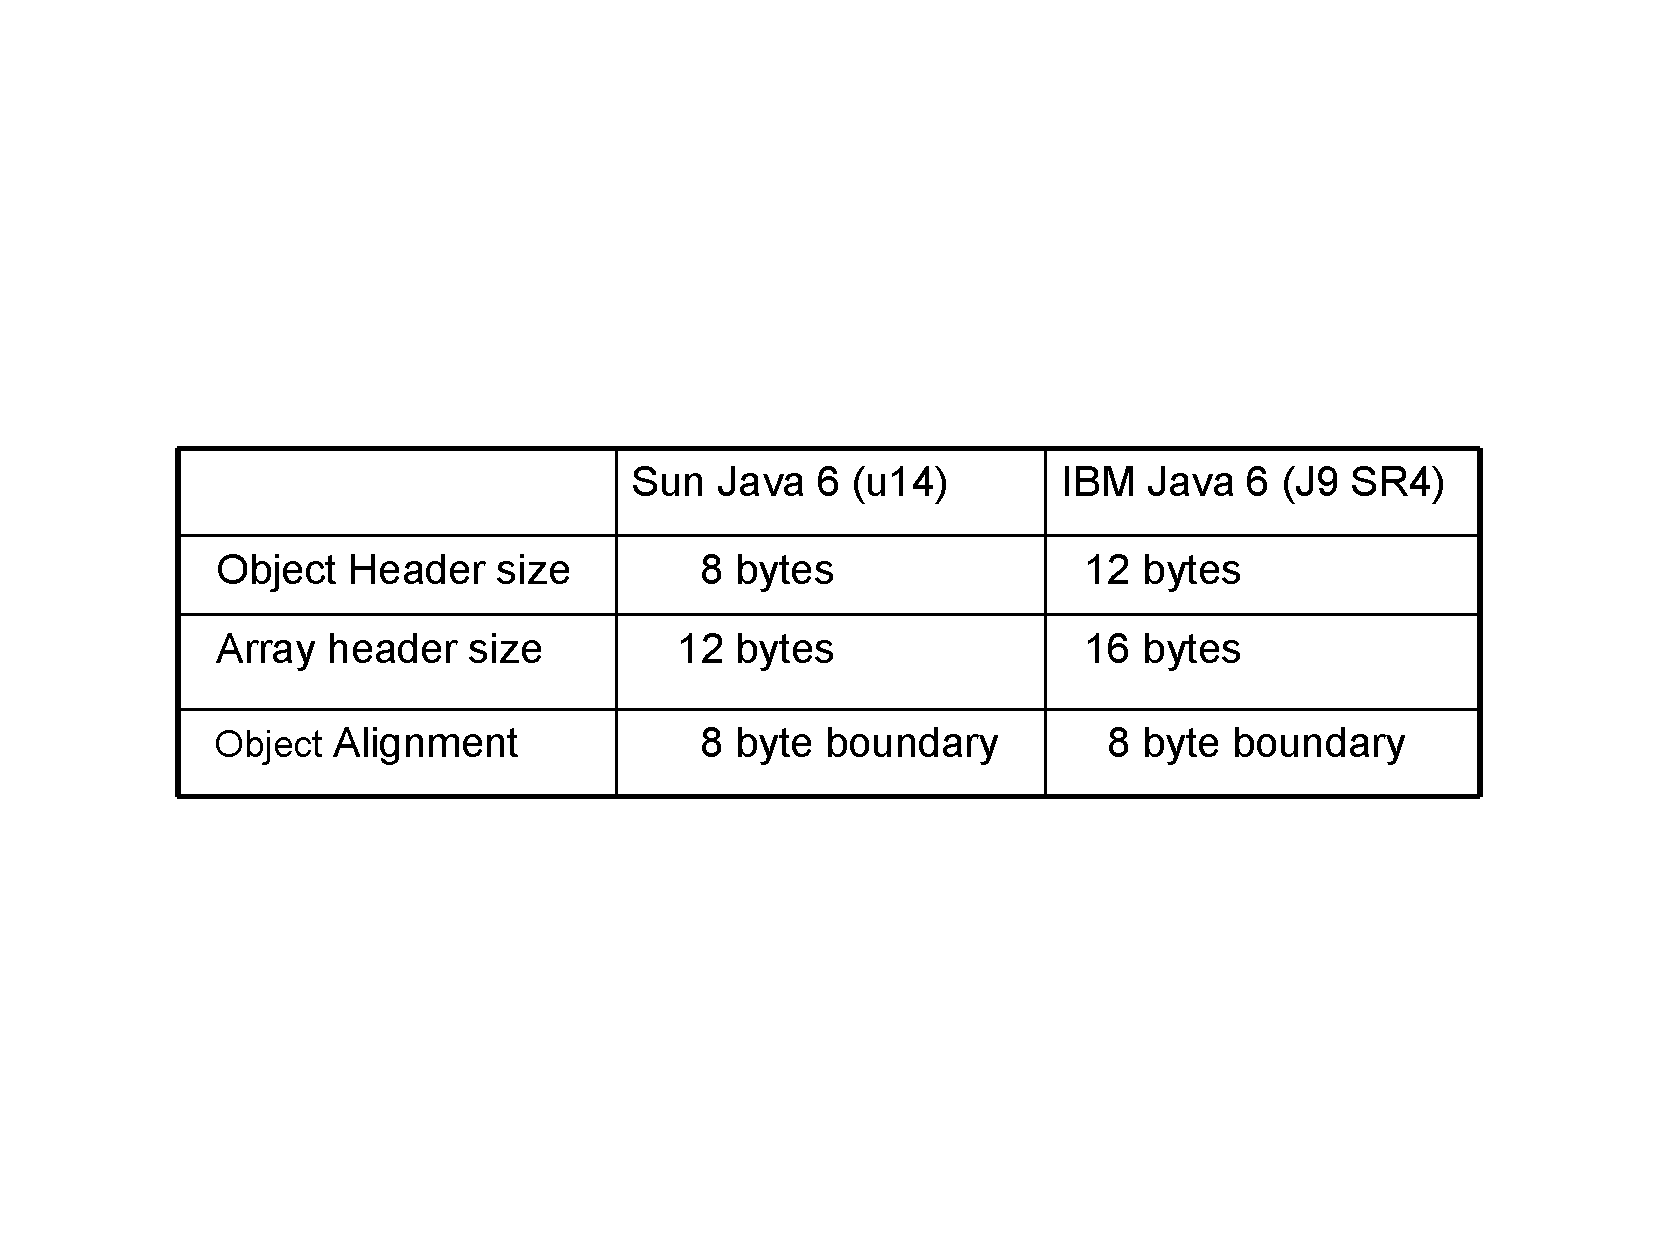
\includegraphics[width=.70\textwidth]{part2/Figures/chapter4/object-overhead.pdf}
 % 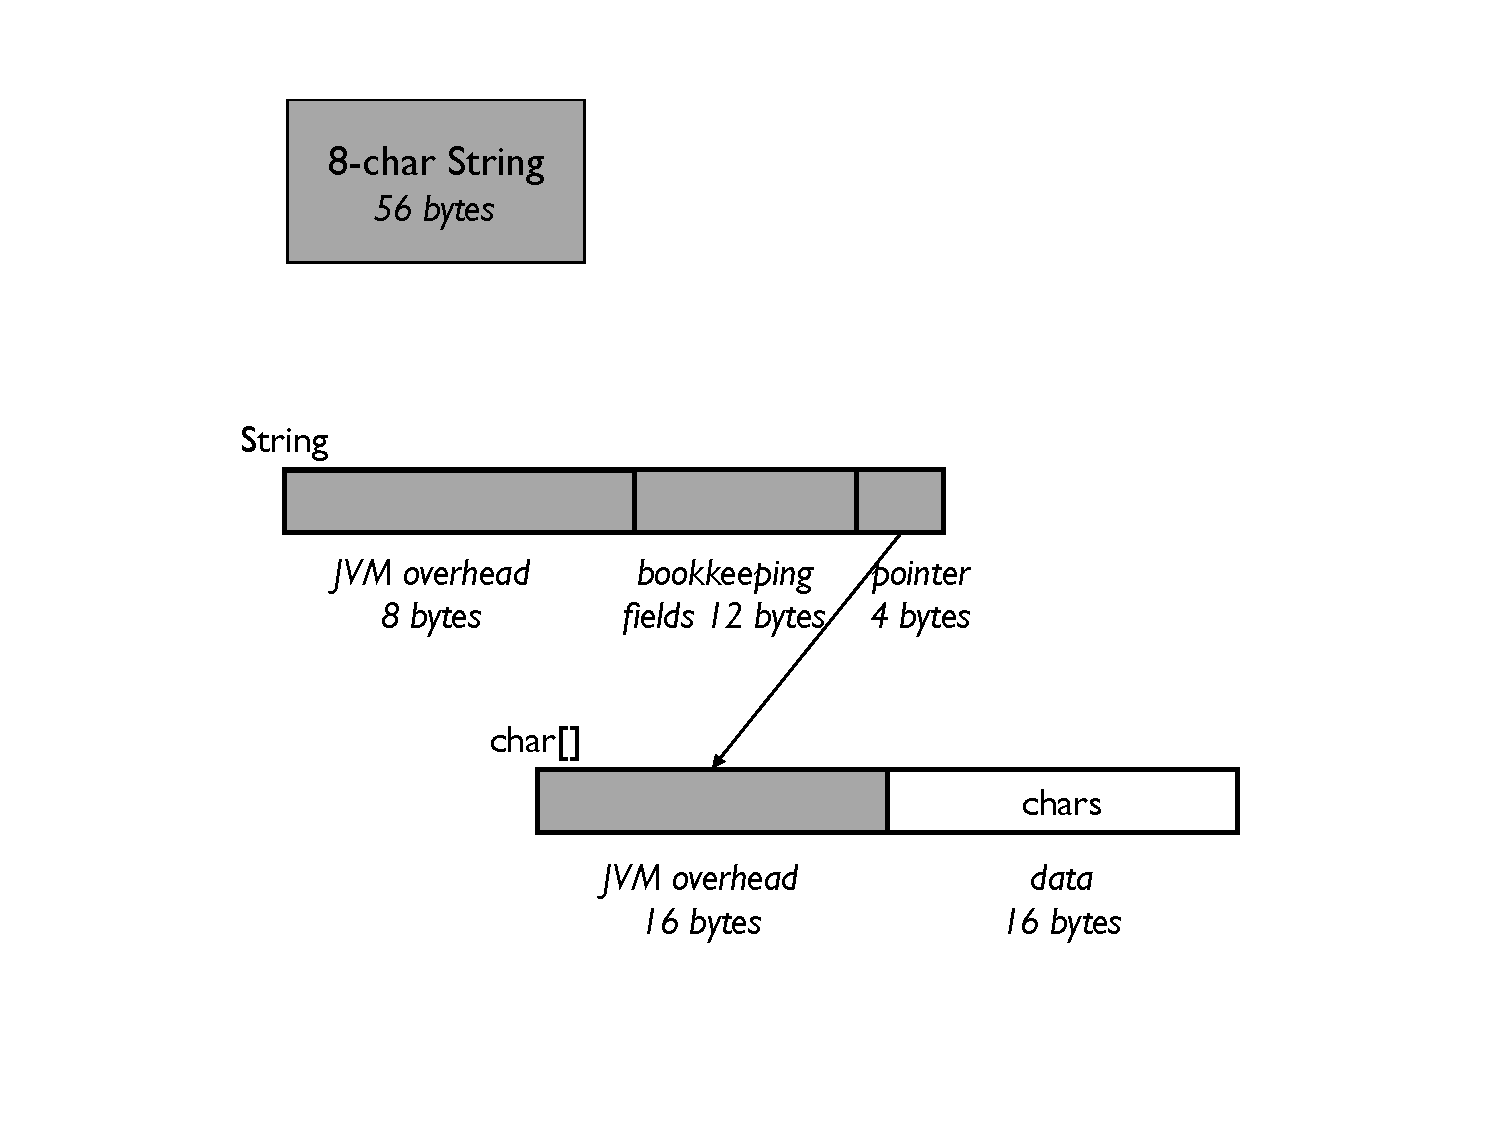
\includegraphics{eight-char-string}
 \begin{tabular}{llll} \toprule
 	 Collection & Fixed Cost & Per-Entry Cost & Default Size \\ \midrule
 	ArrayList & 80 bytes & 4 bytes & 10 entries \\
 	LinkedList &  &  & \\
 	HashMap & 120 bytes & 28 bytes & 16 entries \\
 	HashSet & 136 bytes & 28 bytes & 16 entries \\
 	\bottomrule
 \end{tabular}
  \caption{The cost breakdown of four basic Java standard library collections
  with default size and no entries. The fixed cost includes the memory needed
  for taking the default collection size. The per-entry cost is used to
  determine scalability.}
  \label{tab:collection-costs}
\end{table} 

\section{Properly Sizing Collections}

 Let�s talk a little bit about default sizes and growth policies, and that 
 sort of thing. So this is a little hypothetical experiment here. We�re getting 
 back to the value side of this structure, where you replace the original 
 hashsets by arraylist. He sized them minimally, but having not done that, 
 had he taken the default sizes for the arraylists, it would have cost another
 28\% of overhead, since all the collections, basically are sized pretty 
 aggressively just like StringBuffer is, with this idea of trying to reduce 
 the copying costs and basically assuming that any collections you have are 
 going to grow, and so we�d better pay those costs up front in large chunks, 
 so that you don�t have to constantly pay a reallocation, and copy costs, 
 and it�s really an open question of whether that�s buying us any performance 
 or not, it�s certainly costing people a lot of footprint. One of the common 
 patterns we see is people just take the default size of collections. 
 They just take the constructor, no parameters, and even when they do 
 specify a default size, the collection growth policies are still pretty 
 aggressive. Typically double in size, and there�s even one copy constructor 
 that one of the array list copy constructure, if you hand it a collection and 
 say make me an arraylist out of this, it actually adds 10\% to it, just in
 case you grow this thing. And the typical pattern is you are building some 
 temporary collection to sort something or filter something, and at the last 
 minute you are done with it, and you turn it into an arraylist that you are 
 going to send onto somebody else, and they are not going to modify it again. 
 So there is definitely optimization for some questionable cases in here.

What can you do about this? One is that you can set the initial capacity 
relatively low. If you might be introducing a performance problem then do 
some timing, and see if it�s actually the case. Another thing is if you have 
data modes and many data models have this pattern, where you have a load phase 
vs a usage phase. I load all my data, and I never modify it again. Or maybe 
I�m modifying entries but never adding anything , then you can use  trimToSize. 
Just walk through the whole data model and call trimToSize on every collection. 
You will pay a reallocation and copying cost just once, and that�s it. 


Just a quick look at some of the default sizes. LinkedList, 
it�s not really applicable other than the fact � always comes with an 
extra entry as a sentinel, just to make the coding of LinkedList simpler, 
So you are actually paying 3 entry cost for a 2 element collection. 
ArrayLists, the default size is 10. For some reason, the latest J9, 
in these Harmony classes, which are open source, they�ve upped it to 12, 
and I�m not quite sure why they�ve done that. Actually that�s not really true.
 The default size initially for an empty collection is 0, so they�re still
 allocating the array with 0 size. Where as the Sun and older JVM�s are always 
 allocating 10 element collection. But on the Harmony classes, the new J9, 
 after you add the first element, they jump it to 12. It�s pretty hard not to 
 get those big jumps in these collection classes. HashMap, the default is 16, 
 and HashSet as well, since it�s based on HashMap. So it�s definitely 
 worth setting the default in these cases where you know you have mostly these 
 small collections. 

\section{Avoiding Empty Collections}

A related problem is empty collections, and this is super, super common. 
People are eagerly initializing things, and without realizing that the empty 
collections are pretty costly too. This was the case from JPMorgan 
Chase critsit, that Nick did, and in fact in SessionState, which had all sorts 
of other stuff in it, had these profile objects in it, which were profiles of 
customers, and each of those profiles was a highly delegated design, we saw it 
last week, each one had 40 instances hidden inside that box. 

For those of you who weren�t here last week, this notation is kind of a UML-like 
notation This is a logical data structure and these boxes are hiding other classes.
 The octagonal shaped ones are collections, things implementing relationships. 
 SO profile had quite a few classes inside it, and they all had the same coding 
 pattern in them, where they had these arraylists hanging off of them. 
 In one case it was to track the history of modifications in various fields. 
 In total, each usersession data had 210 empty arraylists hanging off of it, 
 which was rather expensive in this little example here. They were paying  
 8MB in this of just empty arraylists. So what are the remedies here? 
 The simplest thing is to lazily allocate these things. Along with lazy 
 allocation, there�s a nice static method in the collections class, 
called emptyset, where it will return you a pointer to a singleton empty set 
that has all the functionality of a set. EmptySet, EmptyList, EmptyMap, and 
those are great since you can point to them, and the size method will still work,
iterators will still work, all that stuff will still work, and you don�t have 
to allocate an empty collection. The only bad thing with those 2 patterns, 
and you really have to watch out for, is if you give out any references to your 
collections before they�ve been allocated. Because once you give out a 
reference, you expect people to hold on to it, then there�s no way to morph it 
into this other form that�s actually populated. And that�s a serious issue in Java.
 But if you can hide the references within the class, then this is very easy 
 to fix. 

So just a quick look inside the empty collections, you can see that they are not 
all that empty. So all the standard Java collections eagerly allocate their 
subsidiary objects, which means that every empty collection consists of 2 objects, 
2 object headers, a pointer, plus whatever bookkeeping fields they have. 
So you get these rippling effects, you have a really high level code, that�s 
eagerly initializing some package, and it�s eagerly initializing some thing else,
 and eventually it�s initializing some collection, and the collection is doing 
 the same thing; it says, well I�m just going ahead and allocate my array, 
it�s not clear why, it�s either ease of coding, or to avoid an if statement 
check at runtime, it�s not clear. So another area is to see if there�s any 
 performance benefit to this, or is this something that can be changed very 
easily. And juust a quick look at the cost of the empty collections. 
What strikes me � these are the number from both sun and IBM. What strikes
me is that the smallest number here is 48, so there�s certainly no single 
digit anything in Java, but 48 is a pretty high number for something that�s 
empty, if you are going to have a lot of them, and also, there�s a little bit 
of variation, both having to do with whether you�ve made the size default or not, 
and also what kinds of collection class you are choosing.

\section{Fixed Size Collections}

Replacing \class{HashSet} by \class{ArrayList} helps, but it is not the end
of the story. The second problem in Figure~\ref{fig:graph-hashset} is the
implementation of \class{Edge}, which uses an \class{ArrayList} to store the
a target node and an edge label, both \class{Integers}. Even though
\class{ArrayList} is the least expensive collection, its functionality too
general to use for this purposeps6.
 

\section{Replacing Collections With Classes}
